% THIS DOCUMENT IS FOLLOWS THE VOLERE TEMPLATE BY Suzanne Robertson and James Robertson
% ONLY THE SECTION HEADINGS ARE PROVIDED
%
% Initial draft from https://github.com/Dieblich/volere
%
% Risks are removed because they are covered by the Hazard Analysis
\documentclass[12pt]{article}

\usepackage{booktabs}
\usepackage{tabularx}
\usepackage{graphicx}
\usepackage{hyperref}
\usepackage{float}
\graphicspath{ {./res/} }
\hypersetup{
    bookmarks=true,         % show bookmarks bar?
      colorlinks=true,      % false: boxed links; true: colored links
    linkcolor=red,          % color of internal links (change box color with linkbordercolor)
    citecolor=green,        % color of links to bibliography
    filecolor=magenta,      % color of file links
    urlcolor=cyan           % color of external links
}

\newcommand{\lips}{\textit{Insert your content here.}}

%% Comments

\usepackage{color}

\newif\ifcomments\commentstrue %displays comments
%\newif\ifcomments\commentsfalse %so that comments do not display

\ifcomments
\newcommand{\authornote}[3]{\textcolor{#1}{[#3 ---#2]}}
\newcommand{\todo}[1]{\textcolor{red}{[TODO: #1]}}
\else
\newcommand{\authornote}[3]{}
\newcommand{\todo}[1]{}
\fi

\newcommand{\wss}[1]{\authornote{blue}{SS}{#1}} 
\newcommand{\plt}[1]{\authornote{magenta}{TPLT}{#1}} %For explanation of the template
\newcommand{\an}[1]{\authornote{cyan}{Author}{#1}}

%% Common Parts

\newcommand{\progname}{ProgName} % PUT YOUR PROGRAM NAME HERE
\newcommand{\authname}{Team \#, Team Name
\\ Student 1 name
\\ Student 2 name
\\ Student 3 name
\\ Student 4 name} % AUTHOR NAMES                  

\usepackage{hyperref}
    \hypersetup{colorlinks=true, linkcolor=blue, citecolor=blue, filecolor=blue,
                urlcolor=blue, unicode=false}
    \urlstyle{same}
                                


\begin{document}

\title{Software Requirements Specification for \progname: subtitle describing software} 
\author{\authname}
\date{\today}
	
\maketitle

~\newpage

\pagenumbering{roman}

\tableofcontents

~\newpage

\section*{Revision History}

\begin{tabularx}{\textwidth}{p{3cm}p{2cm}X}
\toprule {\textbf{Date}} & {\textbf{Version}} & {\textbf{Notes}}\\
\midrule
Date 1 & 1.0 & Notes\\
Date 2 & 1.1 & Notes\\
\bottomrule
\end{tabularx}

~\\

~\newpage
\section{Purpose of the Project}
\subsection{User Business}

With the world currently facing record high inflation, cost-of-living is at the highest
it has ever been. This affects all daily necessities but is especially true for food and groceries.
As a whole, all households are affected but there is particular financial strain on those with lower-incomes.
As a result, interest in personal finance has grown and become more important in peoples' everyday lives.
To assist these individuals, we are developing an application that can help users better understand their
spending habits and make smarter financial decisions. This application will allow users to
take photos of grocery receipts and track their overall spending, analyze spending trends, and receive
suggestions on cheaper alternatives for purchased grocery items. Overall, we believe this application
will help users stay more informed and reduce grocery spending in the long-term.

\subsection{Goals of the Project}
\begin{itemize}
  \item The created application will help users save money on groceries over time.
  \item The application will provide accurate spending data and suggestions to end users.
\end{itemize}  
\section{Stakeholders}
\subsection{Client}
\lips
\subsection{Customer}
\lips
\subsection{Other Stakeholders}
\lips
\subsection{Hands-On Users of the Project}
\lips
\subsection{Personas}
\lips
\subsection{Priorities Assigned to Users}
\lips
\subsection{User Participation}
\lips
\subsection{Maintenance Users and Service Technicians}
\lips

\section{Mandated Constraints}
\subsection{Solution Constraints}
\lips
\subsection{Implementation Environment of the Current System}
\lips
\subsection{Partner or Collaborative Applications}
\lips
\subsection{Off-the-Shelf Software}
\lips
\subsection{Anticipated Workplace Environment}
\lips
\subsection{Schedule Constraints}
\lips
\subsection{Budget Constraints}
\lips
\subsection{Enterprise Constraints}
\lips

\section{Naming Conventions and Terminology}
\subsection{Glossary of All Terms, Including Acronyms, Used by Stakeholders
involved in the Project}
\lips

\section{Relevant Facts And Assumptions}
\subsection{Relevant Facts}
\lips
\subsection{Business Rules}
\lips
\subsection{Assumptions}
\lips

\section{The Scope of the Work}
\subsection{The Current Situation}
\lips
\subsection{The Context of the Work}
\lips
\subsection{Work Partitioning}
\lips
\subsection{Specifying a Business Use Case (BUC)}
\lips

\section{Business Data Model and Data Dictionary}
\subsection{Business Data Model}
\lips
\subsection{Data Dictionary}
\lips

\section{The Scope of the Product}
\subsection{Product Boundary}
\begin{figure}[H]
  \centering
  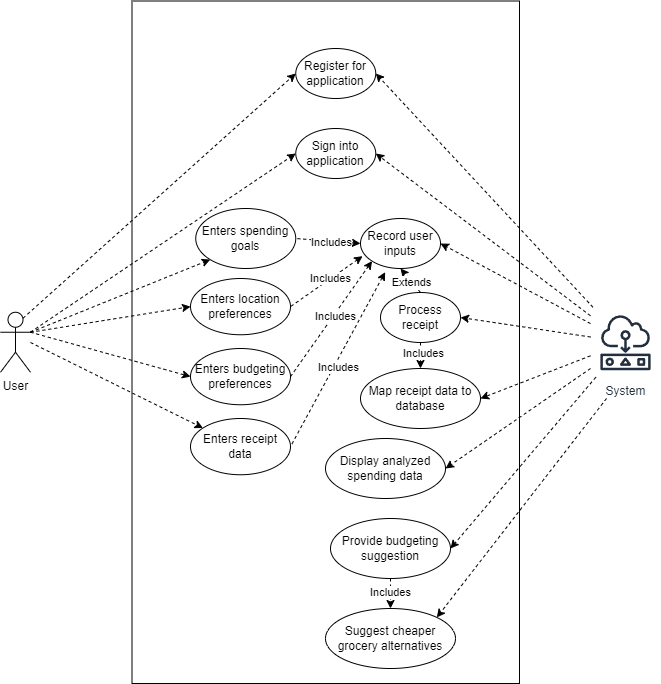
\includegraphics[width=\textwidth]{use_case_diagram}
  \caption{Use Case Diagram}
  \label{fig:use_case_diagram}
\end{figure}

\pagebreak
\subsection{Product Use Case Table}

\begin{table}[H]
  \centering
  \begin{tabular}{ |c|p{3.5cm}|c|p{3.5cm}| } 
  \hline
  \textbf{PUC No} & \textbf{PUC Name} & \textbf{Actor/s} & \textbf{Input/Output} \\ 
  \hline
  1 & Register for an account & User, System & User account data (in), Created user account (out) \\
  \hline
  2 & Sign into application & User, System & User account data (in), Sign in authentication (out) \\
  \hline
  3 & Enter spending goals & User & User spending preferences (in) \\
  \hline
  4 & Enter location preferences & User & User location preferences (in) \\
  \hline
  5 & Enter budgeting preferences & User & User budgeting preferences (in) \\
  \hline
  6 & Enter receipt data & User & Photo of receipt (in) \\
  \hline
  7 & Record user inputs & System & Inputs stored in database (out) \\
  \hline
  8 & Process receipt & System & Receipt data stored in database (out) \\
  \hline
  9 & Map receipt data to database & System & Individual product data properly stored in database (out) \\
  \hline
  10 & Display analyzed spending data & System & Visualized spending data (out) \\
  \hline
  11 & Provide budgeting suggestion & System & Budgeting suggestion (out) \\
  \hline
  12 & Suggest cheaper grocery alternatives & System & Item, price, and location of cheaper alternative (out) \\
  \hline
  \end{tabular}
  \caption{Product Use Case Table}
  \label{tab:productusecasetable}
\end{table}

\pagebreak
\subsection{Individual Product Use Cases (PUC's)}

\textbf{Title:} Register for an account\\
\textbf{Trigger:} User wants to create an account for the application\\
\textbf{Pre-condition:} User has necessary information requested by the system\\
\textbf{Outcome:}
\begin{enumerate}
  \item User enters their email and password when prompted and submits the data.
  \item System validates the data.
  \item If valid, system stores user data in the database and creates the account.
  \item If invalid, system prompts user with an error.
\end{enumerate}

\medskip
\noindent \textbf{Title:} Sign into application\\
\textbf{Trigger:} User wants to sign into their account\\
\textbf{Pre-condition:} User has an account for the application\\
\textbf{Outcome:}
\begin{enumerate}
  \item User enters their email and password when prompted and submits the data.
  \item System looks for any accounts with matching credentials.
  \item If a match is found, system authentication is successful and user is granted application access.
  \item If no match is found, system authentication fails and user is prompted with an error.
\end{enumerate}

\medskip
\noindent \textbf{Title:} Enter spending goals\\
\textbf{Trigger:} User wants to enter their spending goals for the application\\
\textbf{Pre-condition:} User is signed into an account\\
\textbf{Outcome:}
\begin{enumerate}
  \item User enters information regarding their spending objectives and outcomes for application.
  \item System records the entered spending goals into the database.
\end{enumerate}

\medskip
\noindent \textbf{Title:} Enter location preferences\\
\textbf{Trigger:} User wants to enter their location preferences for the application to consider\\
\textbf{Pre-condition:} User is signed into an account\\
\textbf{Outcome:}
\begin{enumerate}
  \item User enters information regarding their current location and preferred area of coverage for the app.
  \item User selects stores they prefer and stores they want to ignore.
  \item System records the entered location preferences into the database.
\end{enumerate}

\medskip
\noindent \textbf{Title:} Enter budgeting preferences\\
\textbf{Trigger:} User wants to enter their budgeting preferences for the application to consider\\
\textbf{Pre-condition:} User is signed into an account\\
\textbf{Outcome:}
\begin{enumerate}
  \item User enters price range and budgeting preferences for the application to consider.
  \item System records the entered budgeting preferences into the database.
\end{enumerate}

\medskip
\noindent \textbf{Title:} Enter receipt data\\
\textbf{Trigger:} User wants to enter a receipt to add new spending data\\
\textbf{Pre-condition:} User is signed into an account and has a receipt to use\\
\textbf{Outcome:}
\begin{enumerate}
  \item User takes a photo of the receipt.
  \item System processes data from the receipt \textit{(see Individual Product
  Use Case for "Process receipt")} and stores data in the database \textit{(see Individual
  Product Use Case for "Map receipt data to database")}.
\end{enumerate}

\pagebreak
\noindent \textbf{Title:} Process receipt\\
\textbf{Trigger:} User enters a photo of a receipt to be analyzed by the application\\
\textbf{Pre-condition:} The receipt photo has already been taken and submitted to the application\\
\textbf{Outcome:}
\begin{enumerate}
  \item System searches the receipt looking for purchase date, time, and location information.
  \item System searches for products purchased and their prices.
  \item Products are mapped \textit{(see Individual Product Use Case for "Map receipt
  data to database")} and purchase data is recorded in the database.
\end{enumerate}

\medskip
\noindent \textbf{Title:} Map receipt data to database\\
\textbf{Trigger:} User enters a photo of a receipt to be analyzed by the application\\
\textbf{Pre-condition:} The receipt has already been processed by the system\\
\textbf{Outcome:}
\begin{enumerate}
  \item System goes through each found product on the receipt and
  checks if it exists in the database.
  \item If an entry in the database exists for the product, the date, time, location,
  and purchase price are recorded in that entry.
  \item If no entry for the product exists in the database, an entry is created and the
  date, time, location, and purchase price are recorded.
\end{enumerate}

\medskip
\noindent \textbf{Title:} Display analyzed spending data\\
\textbf{Trigger:} User wants to check their spending data\\
\textbf{Pre-condition:} The user is logged in and has spending data already entered into the application\\
\textbf{Outcome:}
\begin{enumerate}
  \item The system checks the user's purchases in the database.
  \item The system displays a visual representation of the user's purchase history and
  data is provided on what was purchased and when.
\end{enumerate}

\medskip
\noindent \textbf{Title:} Provide budgeting suggestion\\
\textbf{Trigger:} User exceeds budgeting preferences submitted\\
\textbf{Pre-condition:} The user is logged in and has entered their budgeting preferences into the application\\
\textbf{Outcome:}
\begin{enumerate}
  \item The system analyzes purchase history and compares it to the user's
  budgeting preferences
  \item The system suggests items to stop purchasing and/or cheaper grocery alternatives
  if they exist \textit{(see Individual Product Use Case for "Suggest cheaper grocery
  alternatives")}.
\end{enumerate}

\medskip
\noindent \textbf{Title:} Suggest cheaper grocery alternatives\\
\textbf{Trigger:} A recently purchased item by the user is purchased at a cheaper price\\
\textbf{Pre-condition:} A database entry for the recently purchased item and spending data exist\\
\textbf{Outcome:}
\begin{enumerate}
  \item The system analyzes recent purchase history of the item and purchase location from different users.
  \item If the location is within the current user's location preferences, the item, price and location are
  prompted to the user.
  \item If the location is not within the current user's location preferences, no prompt is created.
\end{enumerate}

\section{Functional Requirements}
\subsection{Functional Requirements}
\lips

\section{Look and Feel Requirements}
\subsection{Appearance Requirements}
\lips
\subsection{Style Requirements}
\lips

\section{Usability and Humanity Requirements}
\subsection{Ease of Use Requirements}
\lips
\subsection{Personalization and Internationalization Requirements}
\lips
\subsection{Learning Requirements}
\lips
\subsection{Understandability and Politeness Requirements}
\lips
\subsection{Accessibility Requirements}
\lips

\section{Performance Requirements}
\subsection{Speed and Latency Requirements}
\lips
\subsection{Safety-Critical Requirements}
\lips
\subsection{Precision or Accuracy Requirements}
\lips
\subsection{Robustness or Fault-Tolerance Requirements}
\lips
\subsection{Capacity Requirements}
\lips
\subsection{Scalability or Extensibility Requirements}
\lips
\subsection{Longevity Requirements}
\lips

\section{Operational and Environmental Requirements}
\subsection{Expected Physical Environment}
\lips
\subsection{Wider Environment Requirements}
\lips
\subsection{Requirements for Interfacing with Adjacent Systems}
\lips
\subsection{Productization Requirements}
\lips
\subsection{Release Requirements}
\lips

\section{Maintainability and Support Requirements}
\subsection{Maintenance Requirements}
\lips
\subsection{Supportability Requirements}
\lips
\subsection{Adaptability Requirements}
\lips

\section{Security Requirements}
\subsection{Access Requirements}
\lips
\subsection{Integrity Requirements}
\lips
\subsection{Privacy Requirements}
\lips
\subsection{Audit Requirements}
\lips
\subsection{Immunity Requirements}
\lips

\section{Cultural Requirements}
\subsection{Cultural Requirements}
\lips

\section{Compliance Requirements}
\subsection{Legal Requirements}
\lips
\subsection{Standards Compliance Requirements}
\lips

\section{Open Issues}
\lips

\section{Off-the-Shelf Solutions}
\subsection{Ready-Made Products}
\lips
\subsection{Reusable Components}
\lips
\subsection{Products That Can Be Copied}
\lips

\section{New Problems}
\subsection{Effects on the Current Environment}
\lips
\subsection{Effects on the Installed Systems}
\lips
\subsection{Potential User Problems}
\lips
\subsection{Limitations in the Anticipated Implementation Environment That May
Inhibit the New Product}
\lips
\subsection{Follow-Up Problems}
\lips

\section{Tasks}
\subsection{Project Planning}
\lips
\subsection{Planning of the Development Phases}
\lips

\section{Migration to the New Product}
\subsection{Requirements for Migration to the New Product}
\lips
\subsection{Data That Has to be Modified or Translated for the New System}
\lips

\section{Costs}
\lips
\section{User Documentation and Training}
\subsection{User Documentation Requirements}
\lips
\subsection{Training Requirements}
\lips

\section{Waiting Room}
\lips

\section{Ideas for Solution}
\lips

\newpage{}
\section*{Appendix --- Reflection}

The information in this section will be used to evaluate the team members on the
graduate attribute of Lifelong Learning.  Please answer the following questions:

\begin{enumerate}
  \item What knowledge and skills will the team collectively need to acquire to
  successfully complete this capstone project?  Examples of possible knowledge
  to acquire include domain specific knowledge from the domain of your
  application, or software engineering knowledge, mechatronics knowledge or
  computer science knowledge.  Skills may be related to technology, or writing,
  or presentation, or team management, etc.  You should look to identify at
  least one item for each team member.
  \item For each of the knowledge areas and skills identified in the previous
  question, what are at least two approaches to acquiring the knowledge or
  mastering the skill?  Of the identified approaches, which will each team
  member pursue, and why did they make this choice?
\end{enumerate}

\end{document}